\documentclass[11pt]{article}
\usepackage{cite}
\usepackage{graphicx}

\begin{document}
\title{Kernel Density Estimation Writeup}
\date{Today}
\maketitle

\section{Kernel density estimation}
The image of the photons on the PMT plane is very complex (see Figure~\ref{fig:distribution}), and so fitting an analytic curve to the data was determined to be infeasible.  As an alternative fitting method, we are trying Kernel Density Estimation \cite{rosenblatt1956}.
\begin{figure}
\centering
\caption{Expected PMT occupancy for one off angle pion.  This geometry has the segmented mirrors and water filling the readout box.\label{fig:distribution}}
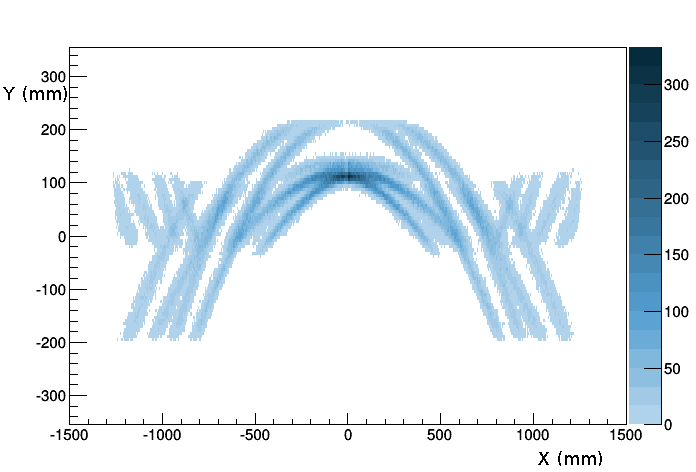
\includegraphics[width=5in]{pngs/fitdirc_ang440_3seg_index_5000MeV_133_pion_dist.png}
\end{figure}
Kernel density estimation works by using a set of monte carlo points to produce a continuous estimate of the value of the pdf that these points are produced from.  The function is obtained by adding the value of a spreading function around each of the provisional points.  While there are several possible options, such as a truncated parabola ("Epanechnikov") or a uniform, for this analysis, a gaussian is chosen as the spreading function mostly due to it's familiarity.  In the early stages of the analysis, several possible functions were tried and little variation was found between them.  Explicitly, the probability at a point $\vec{x}$ with a set of $N_p$ provisional points $\vec{p_i}$ is taken to be the normalized form of:

\begin{equation}
pdf(x) = \sum\limits_{i=1}^{N_p} g(\frac{|p_i-x|}{\lambda})
\end{equation}
\begin{equation}
g(y) = exp(\frac{-y^2}{2})
\end{equation}
Where g is our gaussian spreading function and lambda is optimized to the number of points thrown.  $\lambda$ is also known as the bandwidth, and scales non-trivially with n \cite{SJOS:SJOS445}.

In the case of the DiRC, it is possible to simulate the path of a photon from its creation all the way onto the PMT plane. It is also possible to know within a certain precision the trajectory and energy of an incident particle using the information of the other sub-detectors.  Using the kinematic information, then, one hypothesis for each provisional particle is created and the produced Cerenkov photons are tracked to the PMT plane. Using these provisional points, one pdf for each candidate particle is constructed with kernel density estimation.  This results in 2-3 (depending on the numer of candidates) pdfs per incident particle.

\section{Using the PDFs}
For testing purposes, and with the knowledge that it is the main PID motivation, the pion and the kaon were considered as candidate particles. The study was performed at 4.5 and 5 GeV/c to produce a measurable overlap.  

The produced Cerenkov photons were tracked through the DIRC geometry, and the loglikelihood that they came from each of the provision pdfs was computed.  In order to do this, $N_x$ Photons from each candidate particle were tracked through the simulation to the PMT plane.  These $N_x$ particles were then used to compare the loglikelihood that they cam from one pdf or the other.  If we let $\vec{p_{pion\,i}}$ be the set of provisional particles for the candidate pion and $\vec{p_{kaon\,i}}$ The loglikelihoods were computed as follows:

\begin{equation}
ll_{pion} = \sum\limits_{j=1}^{j=N_x} ln(\sum\limits_{i=1}^{i=N_{pion,p}} g(\frac{|p_{pion,i}-x_j|}{\lambda}))
\end{equation}
Similarly:
\begin{equation}
ll_{kaon} = \sum\limits_{j=1}^{j=N_x} ln(\sum\limits_{i=1}^{i=N_{kaon,p}} g(\frac{|p_{kaon,i}-x_j|}{\lambda}))
\end{equation}

$N_p$ is typically large and currently cosen such that the acheived resolution is on a plateau.  $N_x$ is normalized to 25 for a perpendicular track, as this is what SLAC sees in the test beam

The difference in these loglikelihoods is then reported as the figure of merit to cut on.  The histograms of the loglikelihood difference for a pion versus a kaon is shown here in Figure~\ref{fig:llhistos}.

\begin{figure}
\centering
\caption{$ll_{pion} - ll_{kaon}$ for a non perpendicular track in water.  Pion values shown in red, while kaon values shown in blue. \label{fig:llhistos}}
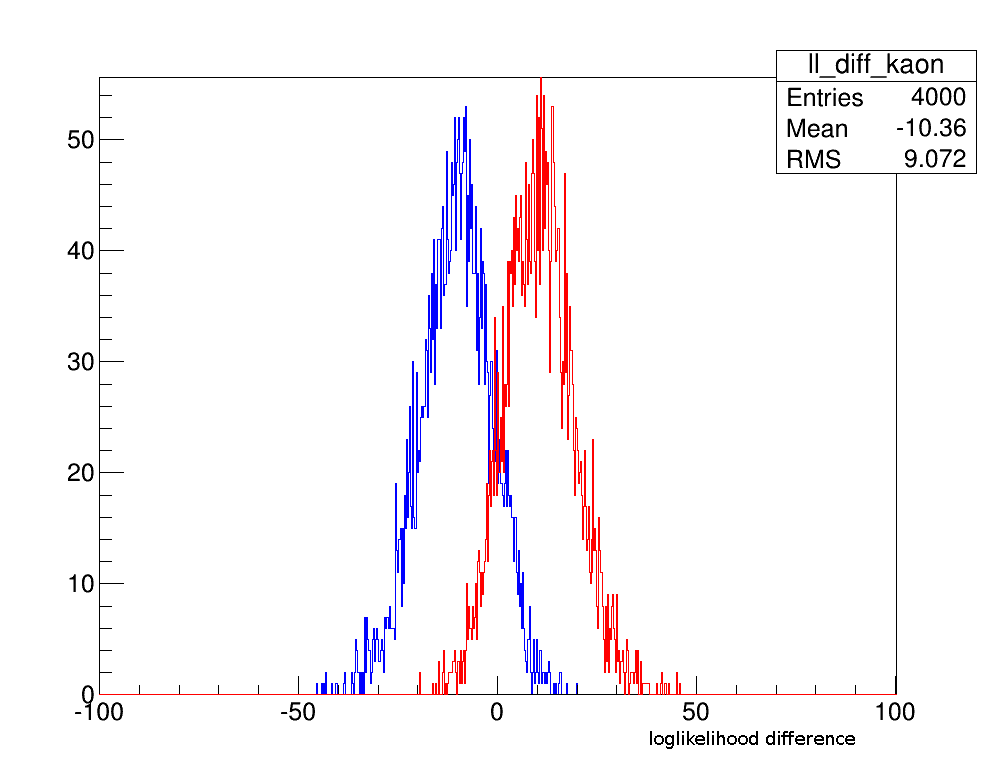
\includegraphics[width=5in]{pngs/ll_diffs.png}
\end{figure}

To quantify the performance, a ROC (Receiver Operating Characteristic) curveis produced as in Figure~\ref{fig:roccurve} and the integral of this ROC curve is compared to the integral of a ROC curve of two ideal gaussians with a mean separation equal to the nominal angular separation of the pion and kaon Cerenkov angles. The gaussians have the same standard deviation, and this sigma is set such that the integrals of the two ROC curves agree.  This number is then quoted as the nominal resolution.
\begin{figure}
\centering
\caption{ROC curve for the histograms in Figure~\ref{fig:llhistos} \label{fig:roccurve}}
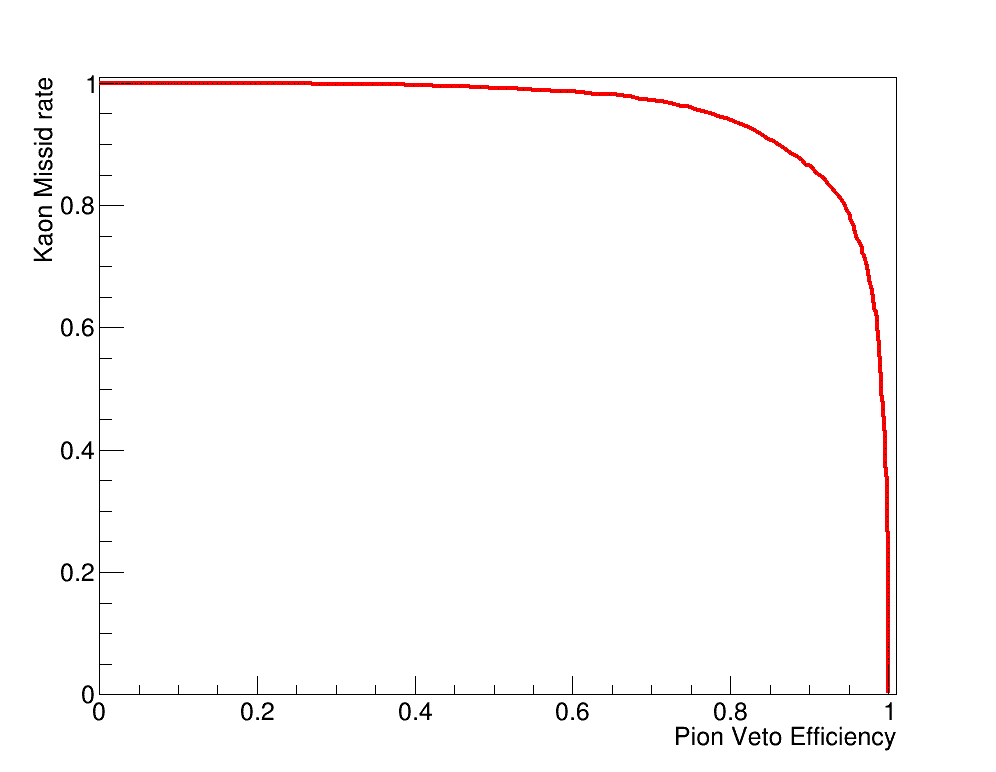
\includegraphics[width=5in]{pngs/roc_curve.png}
\end{figure}

\bibliography{bibliography}{}
\bibliographystyle{plain}
\end{document}